% graphics source https://docs.google.com/presentation/d/111HE56Ow0miZApHPBa18eyPAw8cdslZyBCavoWMix8E
\begin{figure}
\centering
\begin{minipage}{0.47\linewidth}
\centering
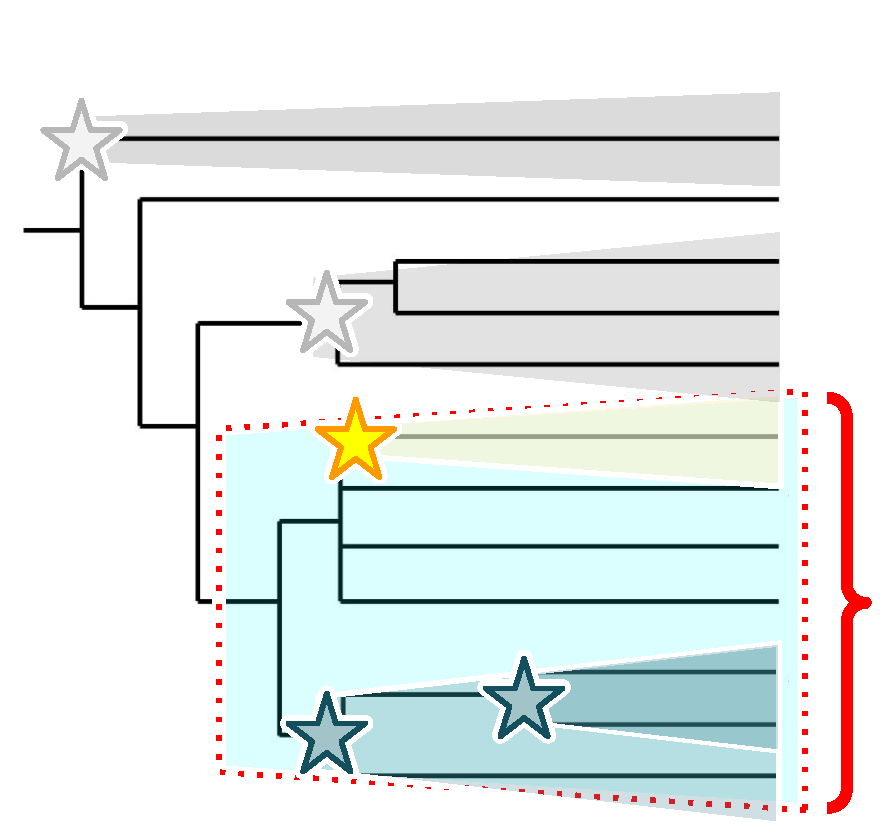
\includegraphics[height=0.75\linewidth,angle=270]{img/comparator-selection-clade}
\subcaption{phylogeny-based}
\label{fig:comparator-selection:clade}
\end{minipage}
~~
\begin{minipage}{0.47\linewidth}
\centering
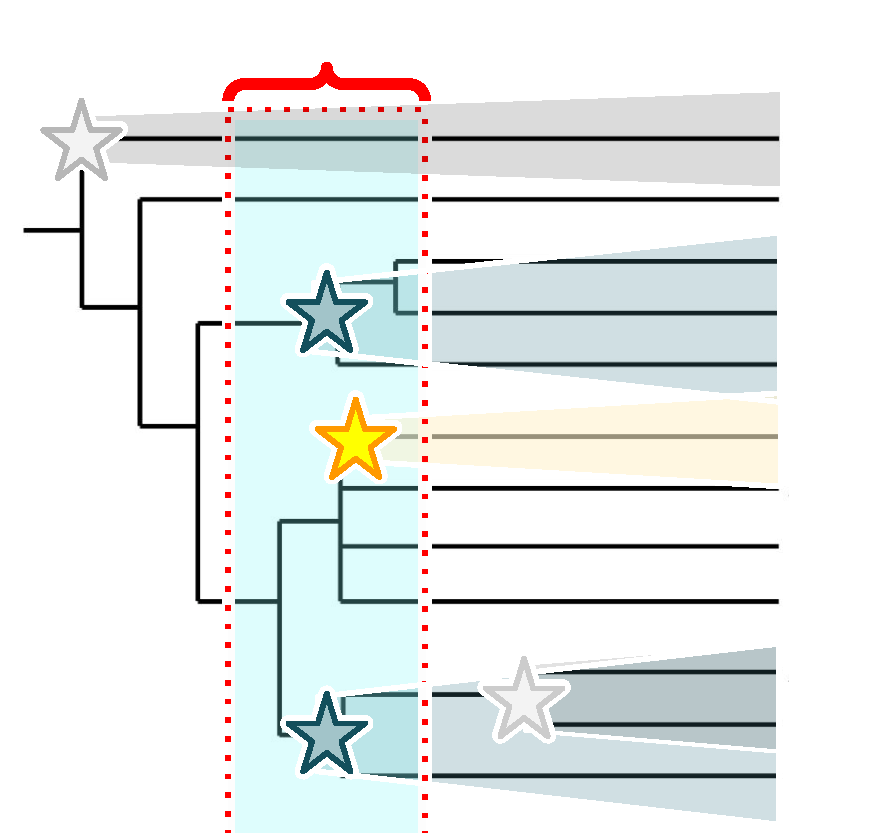
\includegraphics[height=0.75\linewidth,angle=270]{img/comparator-selection-window}
\subcaption{epoch-based}
\label{fig:comparator-selection:window}
\end{minipage}

\begin{minipage}{\linewidth}
\caption{%
\textbf{Strategies for comparator selection.}
\footnotesize Yellow star indicates mutation of interest, teal star indicates mutations defining comparator clades. Grey stars indicate mutations defining clades that are neither the focal clade nor comparator clades.
a) Comparator group is all mutation-defined subclades of a larger clade. b) Comparator group is all mutation-defined clades that originated within a specific timespan.
}
\label{fig:comparator-selection}
\end{minipage}
\vspace{-3ex}
\end{figure}
